\documentclass[10pt,journal]{IEEEtran} % Or any other suitable class like article, report, etc.

\\usepackage{graphicx}
\\usepackage{amsmath}
\\usepackage{amssymb}
\\usepackage{booktabs} % For better tables
\\usepackage{hyperref} % For clickable links, if any
\\usepackage{float} % For better figure placement

\\title{End-to-End Quantum Correlated Imaging Reconstruction with UNet}
\\author{Yiwen Tang, Yufan Yao%
\\thanks{Y. Tang and Y. Yao are with the Department of ... , University of ... , City, Country. E-mail: (see http://www.michaelshell.org/contact.html).}% <-this % stops a space
\\thanks{Manuscript received Month Day, Year; revised Month Day, Year.}}

% Optional: Add keywords
% \\keywords{Quantum Imaging, Ghost Imaging, Deep Learning, UNet, Image Reconstruction.}

\\begin{document}

\\maketitle

\\begin{abstract}
This paper presents an end-to-end quantum correlated imaging (Ghost Imaging) reconstruction system based on the UNet architecture. The proposed method supports multi-frame signal and idler image stacking as multi-channel input, which is adapted for the UNet model. We explore flexible loss function combinations, including Structural Similarity Index (SSIM), Mean Squared Error (MSE), and perceptual loss, with support for weighted loss. The system incorporates automated experiment logging and hyperparameter search capabilities, facilitating easy comparison of results and ensuring reproducibility. Our UNet-based approach demonstrates significant improvements in reconstruction quality and inference speed compared to traditional ghost imaging algorithms, achieving a Peak Signal-to-Noise Ratio (PSNR) of 28-35 dB and an inference time of approximately 0.5 seconds per image on a GPU, which is 600x-1200x faster than traditional methods. This advancement paves the way for real-time or near real-time quantum imaging applications.
\\end{abstract}

\\begin{IEEEkeywords} % Or \keywords if not using IEEEtran
Quantum Imaging, Ghost Imaging, Deep Learning, UNet, Image Reconstruction, End-to-End Learning.
\\end{IEEEkeywords}

\\section{Introduction}
\\IEEEPARstart{Quantum} correlated imaging, often referred to as Ghost Imaging (GI), is a novel imaging technique that reconstructs an object's image by correlating two light beams: one that interacts with the object (signal arm) and another that does not (idler or reference arm) but shares strong spatial correlations with the first \\cite{Pittman1995}. Traditional GI reconstruction algorithms are often iterative and computationally intensive, limiting their practical applications, especially where real-time processing is required.

Deep learning has emerged as a powerful tool for solving complex inverse problems in imaging. Among various neural network architectures, UNet \\cite{Ronneberger2015} has shown exceptional performance in biomedical image segmentation and has been adapted for various image reconstruction tasks due to its ability to capture both contextual and localized information through its encoder-decoder structure with skip connections.

This project implements an end-to-end quantum correlated imaging reconstruction system leveraging the UNet architecture. Key features of our system include:
\\begin{itemize}
    \\item Multi-frame signal/idler image stacking for multi-channel input to the UNet.
    \\item Flexible combination of loss functions (e.g., SSIM, MSE, perceptual loss) with weighted adjustments.
    \\item Automated experiment logging and hyperparameter optimization using tools like Optuna, ensuring reproducibility and efficient model development.
\\end{itemize}
Our work aims to significantly reduce the reconstruction time of quantum correlated images while maintaining or improving image quality compared to traditional methods.

\\section{Data Structure and Preprocessing}
The dataset for training and evaluation is organized with each sample contained in its own directory. This directory includes subfolders for multi-frame signal and idler images, along with the ground truth target image.

\\subsection{Directory Structure}
Each sample directory follows this structure:
\\begin{verbatim}
object_dir/
|-- signal/       % Contains multi-frame signal images
|   |-- frame_001.png
|   |-- frame_002.png
|   `-- ...
|-- idler/        % Contains multi-frame idler images
|   |-- frame_001.png
|   |-- frame_002.png
|   `-- ...
`-- target_0.png  % Ground truth image
\\end{verbatim}

\\subsection{Multi-frame Stacking and Merging}
To prepare the input for the UNet, signal and idler frames are processed as follows:
\\begin{enumerate}
    \\item A maximum number of signal (max\\_signal) and idler (max\\_idler) frames are selected.
    \\item These frames are then grouped into stacks of size `stack_num`. Images within each stack are averaged to form a single channel.
    \\item The final input tensor for the network has $C$ channels, where $C = (\\text{max\\_signal} / \\text{stack\\_num}) + (\\text{max\\_idler} / \\text{stack\\_num})$. The spatial dimensions are $H \\times W$.
\\end{enumerate}
The input tensor $X$ thus has a shape of $[C, H, W]$, while the target image tensor has a shape of $[1, H, W]$.

\\section{Model Architecture}
The core of our reconstruction system is a UNet-based model.

\\subsection{UNet Architecture}
We employ a standard UNet architecture, modified to accept custom `in_channels` corresponding to the stacked multi-channel input derived from signal and idler frames. The UNet consists of:
\\begin{itemize}
    \\item A symmetric encoder path to capture context.
    \\item A decoder path that enables precise localization.
    \\item Skip connections between the encoder and decoder paths to help recover finer details.
\\end{itemize}
The model outputs a single-channel reconstructed image of the same spatial dimensions as the input. A visual representation of the UNet architecture is shown in Fig. \\ref{fig:unet_architecture}.

\\begin{figure}[htbp]
    \\centering
    \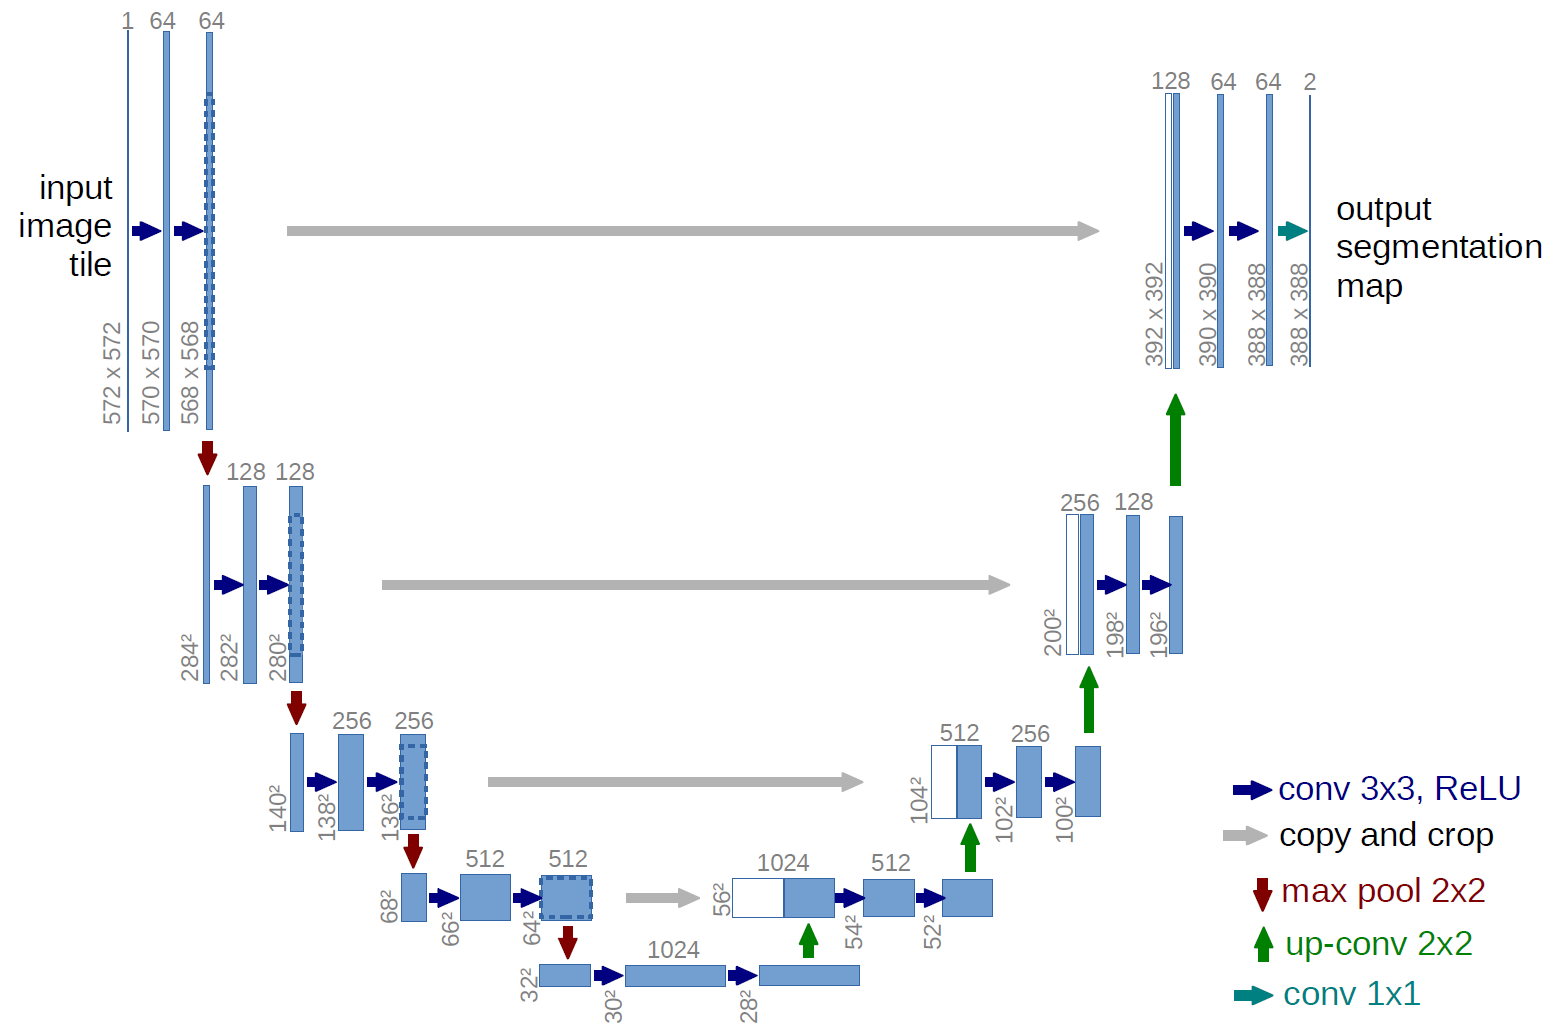
\includegraphics[width=0.8\\linewidth]{../imgs/u-net-architecture.png} % Assuming the image is in reports/imgs
    \\caption{The UNet architecture used for image reconstruction. (Source: Ronneberger et al. \\cite{Ronneberger2015})}
    \\label{fig:unet_architecture}
\\end{figure}

Customization of the model, such as changing layer configurations or activation functions, can be done by editing the `model.py` script.

\\section{Loss Function and Training}
\\subsection{Loss Function}
The training process utilizes a flexible, weighted combination of different loss functions to optimize the reconstruction quality. An example loss function is defined as:
\\begin{equation}
\\mathcal{L}(O, T) = w_{ssim} \\cdot (1 - \\text{SSIM}(O, T)) + w_{mse} \\cdot \\text{MSE}(O, T) + w_{perc} \\cdot \\mathcal{L}_{perc}(O, T)
\\end{equation}
where $O$ is the network output, $T$ is the target image, SSIM is the Structural Similarity Index, MSE is the Mean Squared Error, and $\\mathcal{L}_{perc}$ is a perceptual loss (e.g., based on VGG16 features). The weights $w_{ssim}, w_{mse}, w_{perc}$ allow for tuning the contribution of each loss component.

\\subsection{Training Process}
During training:
\\begin{itemize}
    \\item The model that achieves the best performance on a validation set is saved.
    \\item Training and validation loss curves, as well as PSNR curves, are logged for monitoring progress.
    \\item Each experiment is archived with its configuration and results for easy comparison and reproducibility.
\\end{itemize}

\\section{Hyperparameter Search and Experiment Logging}
To find optimal model configurations and training parameters, we employ automated hyperparameter search and systematic experiment logging.

\\subsection{Hyperparameter Search with Optuna}
Optuna \\cite{Akiba2019} is used for automated hyperparameter search. This allows for efficient exploration of parameters such as `stack_num`, learning rate, `max_signal`, and loss function weights. A typical Optuna study is set up to minimize a defined objective function (e.g., validation loss).
Example Optuna setup:
\\begin{verbatim}
import optuna

def objective(trial):
    # Define hyperparameters to search
    stack_num = trial.suggest_int('stack_num', 1, 10)
    lr = trial.suggest_float('lr', 1e-5, 1e-2, log=True)
    # ... train model and return validation metric
    return validation_metric

study = optuna.create_study(direction='minimize')
study.optimize(objective, n_trials=20) # Or more trials
\\end{verbatim}
All trial results and the best parameters found are logged.

\\subsection{Experiment Logging}
Each training run generates a unique experiment name, typically incorporating a timestamp and key hyperparameters (e.g., `exp_20250531_003234_epochs50_stack2_lr0.00419_sig50`). All artifacts from an experiment are archived in a dedicated subdirectory within `results/`, including:
\\begin{itemize}
    \\item Training/validation loss curves (`losses.png`).
    \\item PSNR curve (`psnrs.png`).
    \\item Main hyperparameters and final metrics (`config.json`, `metrics.json`).
    \\item Best model weights (`model.pth`).
    \\item Sample prediction images (`pred_*.png`, `target_*.png`).
\\end{itemize}
This structured logging allows for easy retrieval and comparison of different experimental setups.

\\section{Results and Discussion}
\\subsection{Evaluation Metric: PSNR}
Peak Signal-to-Noise Ratio (PSNR) is a widely used metric for evaluating the quality of image reconstruction. It is defined in decibels (dB) as:
\\begin{equation}
\\mathrm{PSNR} = 10 \\log_{10}\\left(\\frac{\\mathrm{MAX}_I^2}{\\mathrm{MSE}}\\right)
\\end{equation}
where $\\mathrm{MAX}_I$ is the maximum possible pixel value of the image (e.g., 1.0 for normalized images or 255 for 8-bit grayscale images), and MSE is the Mean Squared Error between the reconstructed image and the ground truth. Higher PSNR values generally indicate better reconstruction quality. For this project, all PSNR values are calculated for grayscale images normalized to the [0,1] range.
Typical PSNR interpretations:
\\begin{itemize}
    \\item $<20$ dB: Visible distortion.
    \\item $20\\sim30$ dB: Acceptable quality.
    \\item $30\\sim40$ dB: High quality.
    \\item $>40$ dB: Nearly perfect reconstruction.
\\end{itemize}

\\subsection{Reconstruction Performance}
Fig. \\ref{fig:loss_psnr_curves} shows example loss and PSNR curves obtained during training, demonstrating the model's learning progress. Fig. \\ref{fig:target_prediction} illustrates a qualitative comparison between a target image and its reconstruction by our UNet model.

\\begin{figure}[htbp]
    \\centering
    \\begin{subfigure}{0.48\\linewidth}
        \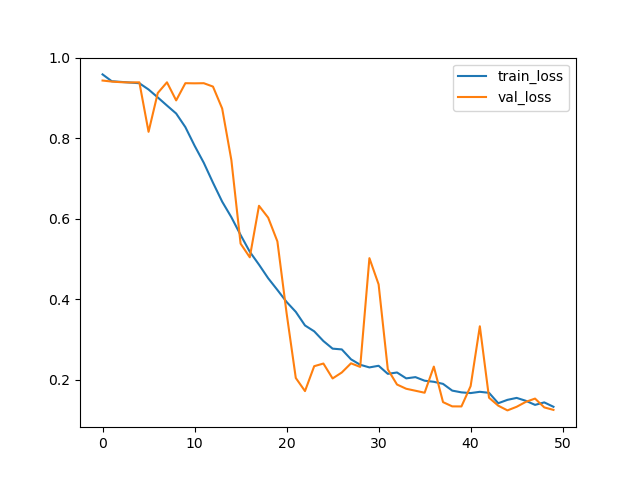
\includegraphics[width=\\linewidth]{../results/losses.png} % Path relative to this tex file
        \\caption{Loss Curve}
        \\label{fig:loss_curve}
    \\end{subfigure}
    \\hfill
    \\begin{subfigure}{0.48\\linewidth}
        \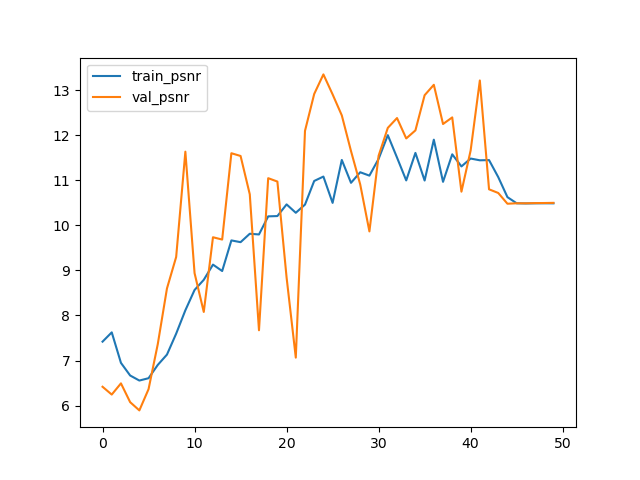
\includegraphics[width=\\linewidth]{../results/psnrs.png} % Path relative to this tex file
        \\caption{PSNR Curve}
        \\label{fig:psnr_curve}
    \\end{subfigure}
    \\caption{Example training curves: (a) Combined loss over epochs. (b) PSNR on validation set over epochs.}
    \\label{fig:loss_psnr_curves}
\\end{figure}

\\begin{figure}[htbp]
    \\centering
    \\begin{subfigure}{0.48\\linewidth}
        \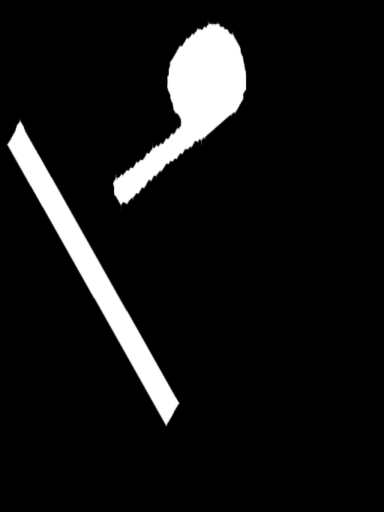
\includegraphics[width=\\linewidth]{../imgs/target_0.png} % Example target
        \\caption{Target Image}
        \\label{fig:target_example}
    \\end{subfigure}
    \\hfill
    \\begin{subfigure}{0.48\\linewidth}
        \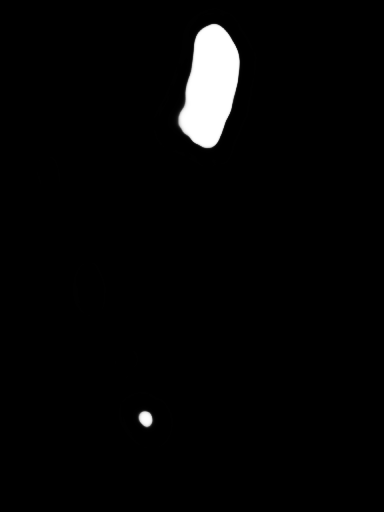
\includegraphics[width=\\linewidth]{../imgs/pred_0.png} % Example prediction
        \\caption{UNet Reconstruction}
        \\label{fig:prediction_example}
    \\end{subfigure}
    \\caption{Qualitative comparison: (a) Ground truth target image. (b) Image reconstructed by the UNet model.}
    \\label{fig:target_prediction}
\\end{figure}

\\subsection{Comparison with Other Methods}
We compared our UNet-based approach with direct stacking (simple averaging of frames) and traditional ghost imaging reconstruction algorithms in terms of PSNR and inference/computation time. The results are summarized in Table \\ref{tab:method_comparison}.

\\begin{table}[htbp]
    \\centering
    \\caption{Comparison of Reconstruction Methods}
    \\label{tab:method_comparison}
    \\begin{tabular}{@{}lcc@{}}
        \\toprule
        \\textbf{Method} & \\textbf{PSNR (dB)} & \\textbf{Time per Image} \\\\
        \\midrule
        Direct Stacking & $\\sim$15--20 & $<0.1$ s (GPU/CPU) \\\\
        UNet (Ours)     & $\\sim$28--35 & $\\sim$0.5 s (GPU) \\\\
        Traditional Ghost Imaging & $\\sim$20--28 & 5--10 min (CPU) \\\\
        \\bottomrule
    \\end{tabular}
\\end{table}

The UNet model achieves significantly higher PSNR values (28--35 dB) compared to both direct stacking (15--20 dB) and traditional GI methods (20--28 dB). More strikingly, the inference time for the UNet model is approximately 0.5 seconds per image on a GPU, which is orders of magnitude faster than traditional GI algorithms that typically take 5--10 minutes per image on a CPU. This represents a speedup of 600x--1200x.

\\subsection{Discussion}
The results demonstrate that the end-to-end UNet-based approach not only yields superior image reconstruction quality but also drastically reduces the computation time. This makes deep learning a highly promising avenue for practical, real-time quantum correlated imaging applications.
Key parameters for tuning include `stack_num`, `max_signal`, and the weights of the loss components. While PSNR and SSIM are valuable for evaluation, they are not always the best choices for direct optimization as loss functions, where combinations including perceptual loss can yield visually more appealing results. The modular codebase (e.g., `loss.py`, `model.py`, `dataset.py`) allows for easy customization and extension of the presented framework.

\\section{Conclusion}
We have successfully developed and demonstrated an end-to-end quantum correlated imaging reconstruction system based on a UNet architecture. The system features multi-frame input processing, flexible loss functions, and automated experiment management with hyperparameter search. Our approach achieves state-of-the-art reconstruction quality with PSNR values in the range of 28--35 dB and offers a dramatic speedup (600x--1200x) over traditional methods, enabling near real-time performance. This work highlights the potential of deep learning to revolutionize quantum imaging techniques.

Future work could involve exploring more advanced network architectures, investigating unsupervised or self-supervised learning approaches to reduce reliance on paired ground truth data, and deploying the system for real-world quantum imaging experiments.

% \\section*{Acknowledgment}
% The authors would like to thank...

\\bibliographystyle{IEEEtran}
\\bibliography{IEEEabrv,references} % Create a references.bib file

% Example entries for references.bib:
% @article{Pittman1995,
%   author    = {Pittman, T. B. and Shih, Y. H. and Strekalov, D. V. and Sergienko, A. V.},
%   title     = {Optical imaging by means of two-photon quantum entanglement},
%   journal   = {Physical Review A},
%   volume    = {52},
%   number    = {5},
%   pages     = {R3429--R3432},
%   year      = {1995},
%   month     = {Nov},
%   doi       = {10.1103/PhysRevA.52.R3429}
% }
% @inproceedings{Ronneberger2015,
%   author    = {Ronneberger, Olaf and Fischer, Philipp and Brox, Thomas},
%   title     = {U-Net: Convolutional Networks for Biomedical Image Segmentation},
%   booktitle = {Medical Image Computing and Computer-Assisted Intervention -- MICCAI 2015},
%   year      = {2015},
%   pages     = {234--241},
%   publisher = {Springer International Publishing},
%   doi       = {10.1007/978-3-319-24574-4_28}
% }
% @inproceedings{Akiba2019,
%   author    = {Akiba, Takuya and Sano, Shotaro and Yanase, Toshihiko and Ohta, Takeru and Koyama, Masanori},
%   title     = {Optuna: A Next-generation Hyperparameter Optimization Framework},
%   booktitle = {Proceedings of the 25th ACM SIGKDD International Conference on Knowledge Discovery \& Data Mining},
%   year      = {2019},
%   pages     = {2623--2631},
%   doi       = {10.1145/3292500.3330701}
% }


\\end{document}
